\begin{figure}[t]\centering
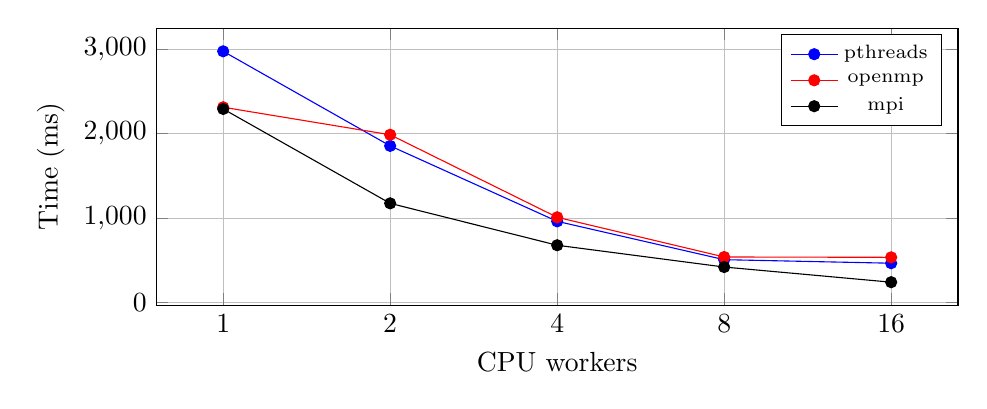
\begin{tikzpicture}\begin{axis}[width=0.97\columnwidth,height=5.1cm,xlabel={CPU workers},ylabel={Time (ms)},xmode=log,log basis x=2,xtick={1,2,4,8,16},xticklabels={1,2,4,8,16},legend style={font=\scriptsize},grid=major]
\addplot[blue,mark=*] coordinates {(1,2974.2846956666667) (2,1854.6393073333334) (4,961.5561986666667) (8,507.641633) (16,465.71177266666666)};\addlegendentry{pthreads}
\addplot[red,mark=*] coordinates {(1,2312.296442) (2,1986.5161413333333) (4,1009.533049) (8,539.393819) (16,535.5408663333333)};\addlegendentry{openmp}
\addplot[black,mark=*] coordinates {(1,2291.9239063333334) (2,1174.5926776666668) (4,678.410175) (8,420.45948100000004) (16,241.17197033333335)};\addlegendentry{mpi}
\end{axis}\end{tikzpicture}
\caption{Large-dataset CPU classification times on Athena's EPYC 7742 node. Three-run means are shown; individual values in the appendix expose run-to-run variation.}\label{fig:cpu}
\end{figure}
